\chapter{Ecossistema Hadoop}
\label{cap:eco}

Os capítulos anteriores abordaram os principais componentes do Hadoop: o sistema de arquivos distribuídos HDFS e o \textit{framework} \textit{MapReduce}. Estes podem ser considerados o núcleo de todo o sistema, porém o Hadoop também é composto por um conglomerado de projetos que fornecem serviços relacionados a computação distribuída em larga escala, formando o ecossistema Hadoop. A tabela \ref{tab-eco} apresenta alguns projetos que estão envolvidos neste contexto.

\begin{savenotes}
\begin{table}[!ht]
\begin{center}
  \begin{tabular}{|p{3cm}|p{7cm}|}
	\hline
	Projeto & Descrição
	\\ \hline
	Common & Conjunto de componentes e interfaces para sistemas de arquivos distribuídos e operações de Entrada/Saída.
	\\ \hline
	HDFS & Sistema de arquivos distribuídos executado sobre clusters com máquinas de baixo custo
	\\ \hline
	\textit{MapReduce} & \textit{Framework} para processamento distribuído de dados, aplicado em \textit{clusters} com máquinas de baixo custo.
	\\ \hline
	Pig\footnote{\url{http://pig.apache.org/}} & Linguagem de procedimentos de alto nível para grandes bases de dados. Executada em \textit{clusters} HDFS e \textit{MapReduce}.
	\\ \hline
	Hive\footnote{\url{http://hive.apache.org/}} & Um \textit{data warehouse} distribuído. Gerencia arquivos no HDFS e provê linguagem de consulta baseada em SQL.
	\\ \hline
	HBase\footnote{\url{http://hbase.apache.org/}} & Banco de dados distribuído orientado a colunas. Utiliza o HDFS para armazenamento dos dados.
	\\ \hline
	ZooKeeper\footnote{\url{http://zookeeper.apache.org/}} & Coordenador de serviços distribuídos.
	\\ \hline
	Flume\footnote{\url{https://flume.apache.org/}} & Ferramenta para transferência de dados entre diferentes fontes.
	\\ \hline
	Sqoop\footnote{\url{http://sqoop.apache.org/}} & Ferramenta para mover dados entre banco relacionais e o HDFS.
	\\ \hline
  \end{tabular}
  \captionsetup{justification=centering}
  \caption[Ecossistema Hadoop]{Ecossistema Hadoop
  \protect\linebreak Fonte: Adaptado de \cite{white2012} e \cite{shvachko2010}}
\label{tab-eco}
\end{center}
\end{table}
\end{savenotes}

Apesar do Hadoop apresentar uma boa alternativa para processamento em larga escala, ainda existem algumas limitações em seu uso. Como discutido anteriormente, o HDFS foi projetado de acordo com o padrão \textit{write-once}, \textit{read-many-times}, desta forma, não há acesso randômico para operações de leitura e escrita. Outro aspecto negativo se dá pelo baixo nível requerido para o desenvolvimento neste tipo de ambiente. Segundo \citeonline{thusoo2009}, a utilização do \textit{framework} \textit{MapReduce} faz com que programadores implementem aplicações difíceis de realizar manutenção e reuso de código,

Alguns dos projetos do ecossistema citado na tabela \ref{tab-eco} foram criados justamente para resolver estes problemas. Desta maneira, utilizam-se do Hadoop para prover serviços com um nível de abstração maior para o usuário. Neste capítulo, discute-se sobre a ferramenta de \textit{data warehouse} distribuído Hive e também sobre o banco de dados orientado a colunas HBase. No capítulo \ref{cap:proposta}, durante a especificação do estudo de caso, serão abordadas as ferramentas Flume e Sqoop, utilizadas, principalmente, para transferência de dados entre o \textit{cluster} Hadoop e outros ambientes.

\section{Hive}

Antes de iniciar a discussão proposta por esta seção, será apresentado o conceito de \textit{data warehouse}. \citeonline{inmon2005} define \textit{data warehouse} como uma coleção de dados integrados, orientados por assuntos, não voláteis e variáveis com o tempo, na qual oferece suporte ao processo de tomada de decisões. Uma arquitetura deste tipo armazena, de forma centralizada, os dados granulares de uma determinada empresa e permite uma análise elaborada destas informações que são coletadas de diferentes fontes.

De acordo com \citeonline{kimball2013}, um dos principais objetivos de um \textit{data warehouse} é facilitar o acesso à informação contida nos dados armazenados, de forma que não apenas os desenvolvedores sejam capazes de interpretar, mas também usuários com uma visão voltada para o negócio e não para aspectos técnicos de implementação. Este tipo de solução estrutura os dados para auxiliar a realização de consultas e análises.

O Apache Hive é uma ferramenta \textit{open-source} para \textit{data warehousing} construída no topo da arquitetura  Hadoop \cite{thusoo2009}. Este projeto foi desenvolvido pela equipe do Facebook para atender as necessidades de análise do grande volume de informações geradas diariamente pelos usuários desta rede social. A motivação encontrada para a criação deste projeto se deu pelo crescimento exponencial da quantidade de dados processados pelas aplicações de BI, tornando as soluções tradicionais para \textit{data warehouse} inviáveis, tanto no aspecto financeiro, como computacional.

Além das aplicações de BI utilizadas internamente pelo Facebook, muitas funcionalidades providas pela empresa utilizam processos de análise de dados. Até o ano de 2009 a arquitetura para este requisito era composta por um \textit{data warehouse} que utilizava uma versão comercial de um banco de dados relacional. Entre os anos de 2007 e 2009 a quantidade de dados armazenados cresceu de forma absurda, passando de 17 terabytes para 700 terabytes. Alguns processos de análise chegavam a demorar dias, quando executados nestas condições.

Segundo \citeonline{thusoo2009}, para resolver este grave problema a equipe do Facebook optou por adotar o Hadoop como solução. A escalabilidade linear, capacidade de processamento distribuído e habilidade de ser executado em \textit{clusters} compostos por hardwares de baixo custo motivaram a migração de toda antiga infraestrutura para esta plataforma. O tempo de execução dos processos de análise que antes podiam levar dias foi reduzido para apenas algumas horas.

Apesar desta solução encontrada, o uso do Hadoop exigia que os usuário desenvolvessem programas \textit{MapReduce} para realizar qualquer tipo de análise, até mesmo pequenas tarefas, por exemplo, contagem de linhas e cálculos de médias aritméticas. Esta situação prejudicava a produtividade da equipe, pois nem todos eram familiarizados com esse paradigma, e em muitos casos era necessário apenas realizar análises que seriam facilmente resolvidas com o uso de uma linguagem de consulta. De acordo com \citeonline{thusoo2009}, o Hive foi desenvolvido para facilitar este processo introduzindo os conceitos de tabelas, colunas e um subconjunto da linguagem SQL ao universo Hadoop, mantendo todas as vantagens oferecidas por esta arquitetura.

\subsection{Características}

Como dito anteriormente, o Hive utiliza o conceito de tabelas para registrar as informações em sua base de dados. Cada coluna está associada a um tipo específico que pode ser primitivo ou complexo. Segundo \citeonline{thusoo2009}, quando um registro é inserido os dados não precisam ser convertidos para um formato customizado, como ocorre em bancos de dados convencionais, apenas utiliza-se a serialização padrão do Hive, desta forma, economiza-se tempo em um contexto que envolve um grande volume de dados. \citeonline{white2012} afirma que esta abordagem pode ser denominada como \textit{schema on read}, pois não há verificação do esquema definido com os dados que estão sendo armazenados, apenas ocorrem operações de cópia ou deslocamento, diferentemente de como acontece em bancos de dados relacionais. Os tipos primitivos são apresentados na tabela \ref{tab-hive-types}.

\begin{table}[!ht]
\begin{center}
  \begin{tabular}{|p{3cm}|p{4cm}|p{4cm}|}
  \hline
  Categoria & Tipo de dado & Descrição \\ 
  \hline
  \multirow{6}{*}{Primitivo} 
  & Inteiro 		& Permite a declaração de inteiros de 1 byte até 8 bytes \\ \cline{2-3} 
  & Ponto flutuante 	& Permite variáveis do tipo float ou de dupla precisão (double) \\ \cline{2-3}
  & Booleano		& Verdadeiro ou falso \\ \cline{2-3}
  & String 		& \textit{Array} de caracteres \\ \cline{2-3}
  & Binário 		& \textit{Array} de caracteres \\ \cline{2-3}
  & \textit{Timestamp} 		& Indica uma marcação temporal com precisão de nanosegundos \\
  \hline
  \multirow{3}{*}{Complexo} 
  & \textit{Array} 		& Lista ordenada de elementos do mesmo tipo \\ \cline{2-3} 
  & \textit{Map} 		& Estrutura associativa que associa uma chave a um tipo especifico de valores \\ \cline{2-3}
  & \textit{Struct}		& Estrutura que é composta por um conjunto de campos associados a um tipo específico \\
  \hline
  \end{tabular}
  \captionsetup{justification=centering}
  \caption[Tipos de dados - Hive ]{Tipos de dados - Hive
  \protect\linebreak Fonte: Adaptado de \cite{white2012}}
\label{tab-hive-types}
\end{center}
\end{table}
\FloatBarrier

O Hive disponibiliza uma linguagem para consultas denominada HiveQL, na qual é composta por um subconjunto do padrão SQL com adaptações para grandes bases de dados. Segundo \citeonline{white2012}, esta abordagem foi fortemente influenciada pela linguagem de consulta presente no banco de dados relacional MySQL\footnote{\url{http://www.mysql.com/}}. Utilizando este recurso usuários podem realizar análises em grandes volumes de informações sem a necessidade de desenvolver aplicações \textit{MapReduce}, apenas com o conhecimento em SQL. O quadro \ref{cod-hiveql} apresenta um exemplo de comando escrito em HiveQL para criar uma tabela, composta por colunas de tipos primitivos e complexos.

\lstinputlisting[frame=single,
		label=cod-hiveql,
		style=abnt,
		caption={[Comando HiveQL]Comando HiveQL
		\protect\linebreak Fonte: Autor}]
		{quadros/hiveql.sql}
\FloatBarrier

\subsection{Arquitetura}

Na seção anterior, foi apresentado o modelo de dados utilizado pelo Hive, onde a organização se dá pelo uso de tabelas compostas por colunas, onde os registros são incluídos em linhas. Estes itens são apenas uma representação lógica, o armazenamento físico dos dados é realizado no HDFS. De acordo com \citeonline{thusoo2009}, o mapeamento entre estas abordagens pode ser identificado a seguir:

\begin{itemize}

  \item \textbf{Tabelas:} Uma tabela representa um diretório no HDFS, todas as informações são registradas dentro deste ficheiro.
  \item \textbf{Partições:} O usuário pode particionar uma tabela de acordo com uma ou mais colunas. Assim, cada partição é registrada em um subdiretório do ficheiro onde está localizado a tabela.
  \item \textit{\textbf{Buckets:}} Um \textit{bucket} é o arquivo onde os registros da tabela de fato são armazenados. Estas estruturas representam o último nível desta árvore de diretórios de uma tabela no HDFS.

\end{itemize}

Como discutido no capítulo \ref{cap:mapreduce-devel}, o Hadoop permite armazenar aquivos de diversos formatos, que podem ser inclusive customizados através da interface \textit{InputFormat}. De acordo com \citeonline{thusoo2009}, o Hive não impõe nenhum restrição quanto ao formato escolhido para gravar os \textit{buckets} no HDFS, inclusive permite que no comando HiveQL o usuário especifique este parâmetro. Isto pode ser feito com o uso da cláusula \textit{STORED AS}. O quadro \ref{cod-hiveql-create} apresenta um comando para criação de uma tabela, na qual deve ser armazenada fisicamente como um arquivo binário, de acordo com as classes \textit{SequenceFileInputFormat} e \textit{SequenceFileOutputFormat}.


\lstinputlisting[frame=single,
		label=cod-hiveql-create,
		style=abnt,
		caption={[Uso da cláusula STORED AS]Uso da cláusula STORED AS
		\protect\linebreak Fonte: \cite{thusoo2009}}]
		{quadros/hiveql-storeas.sql}
\FloatBarrier

O uso da ferramenta Hive é disponibilizado através de três serviços que permitem usuários executarem comandos no formato HiveQL. Uma das opções é o uso de uma interface em linha de comando, similar a um terminal Unix, assim como ocorrem em bancos de dados relacionais, como por exemplo, MySQL e PostgreSQL\footnote{\url{http://www.postgresql.org/}}. Segundo \citeonline{thusoo2009}, as consultas também podem ser submetidas através do uso de um serviço \textit{web} ou com a utilização de \textit{drivers} de conexão JDBC/ODBC\footnote{} para a interação com outras aplicações. Estes serviços estão presentes no topo pilha de tecnologias do Hive e podem ser observados na figura \ref{fig-hive}, onde é apresentada a arquitetura geral da plataforma.

\begin{figure}[ht!]
	\centering
	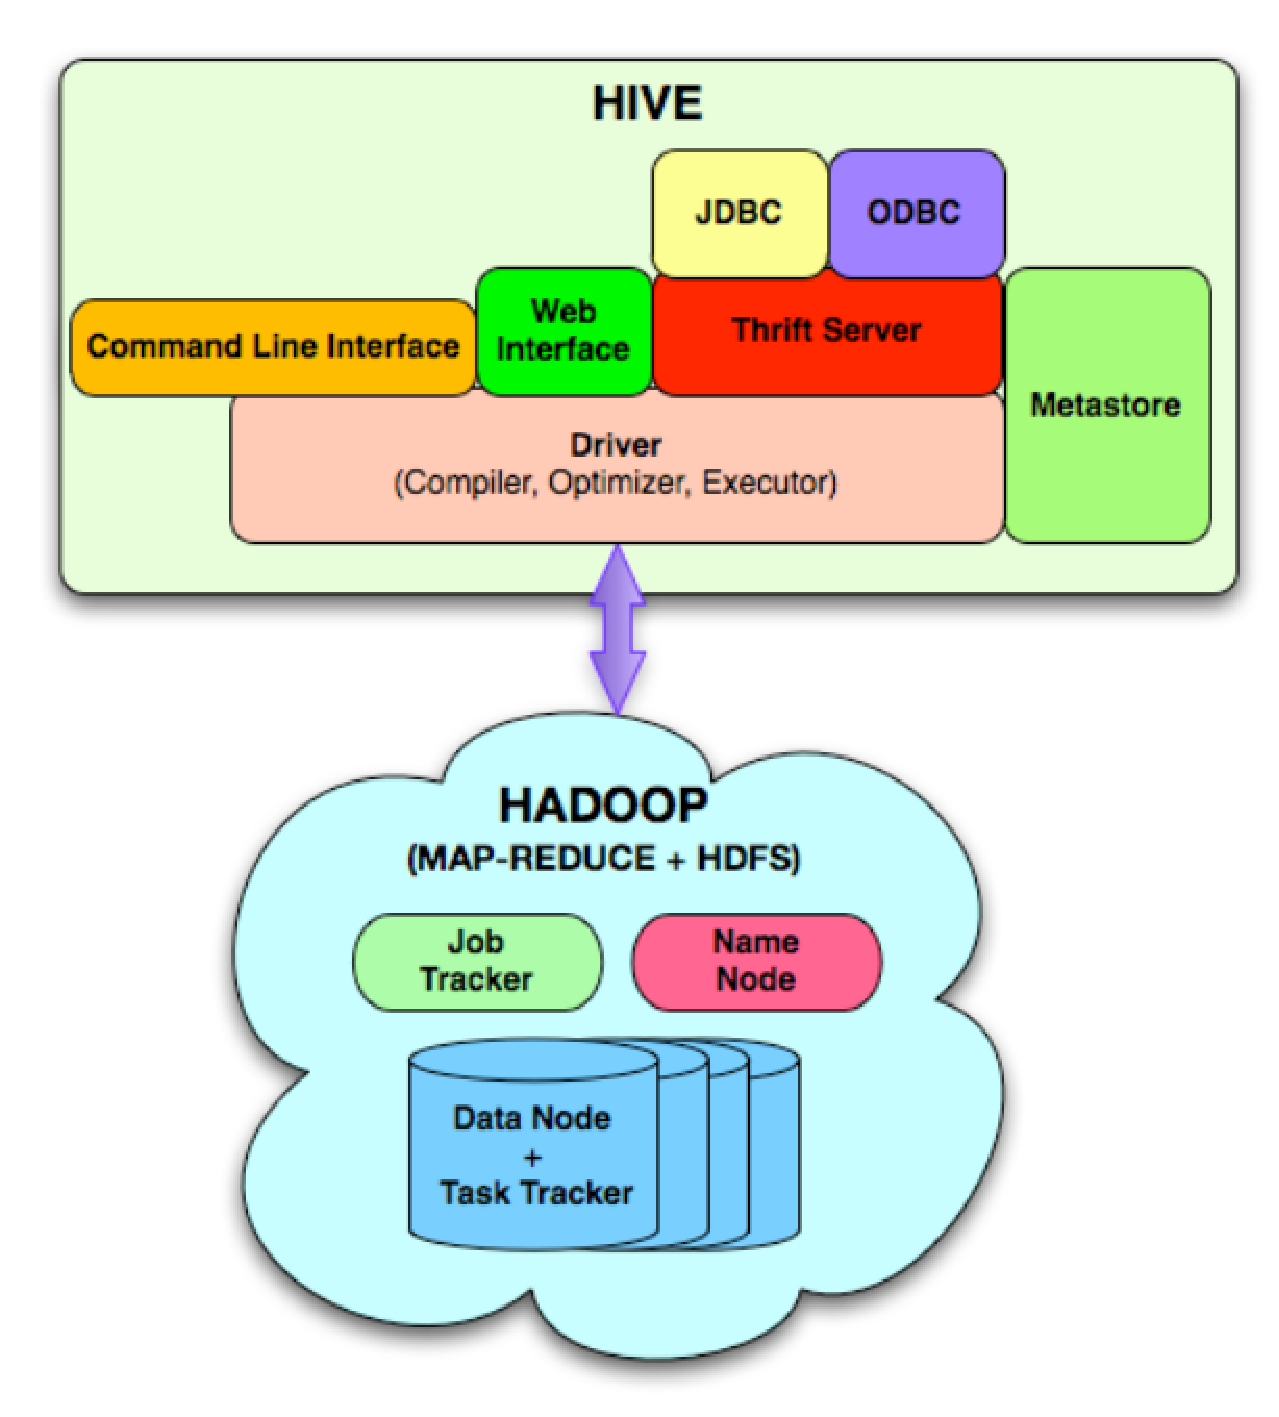
\includegraphics[keepaspectratio=true,scale=0.5]
	  {figuras/hive.eps}
	\caption[Arquitetura Hive]{Arquitetura Hive
	\protect\linebreak Fonte: \cite{thusoo2009}}
	\label{fig-hive}
\end{figure}
\FloatBarrier

O grande diferencial está no componente denominado \textit{driver}, o qual está presente no núcleo da arquitetura. Nesta etapa, o comando HiveQL é compilado e convertido para um grafo acíclico, onde cada nó é representado por um \textit{MapReduce} \textit{job}. São realizadas otimizações e a ordenação topológica, resultando em uma sequência de \textit{jobs} que serão executados no \textit{cluster} Hadoop. Um comando HiveQL pode gerar vários \textit{MapReduce} \textit{jobs}, que são intercalados para se obter o resultado final.


\section{HBase}

Os bancos de dados relacionais sempre desempenharam um papel importante no \textit{design} e implementação dos negócios da maioria das empresas. As necessidades para este contexto sempre envolveram o registro de informações de usuários, produtos, entre inúmeros exemplos. Este tipo de arquitetura oferecida pelos SGBDs foram construídas de acordo com o modelo de transações definido pelas propriedades ACID. Segundo \citeonline{george2011}, desta forma, é possível garantir que os dados sejam fortemente consistentes, o que parece ser um requisito bastante favorável. Esta abordagem funciona bem enquanto os dados armazenados são relativamente pequenos, porém o crescimento desta demanda pode ocasionar sérios problemas estruturais.

De acordo com \citeonline{george2011}, os bancos de dados relacionais não estão preparados para análise de grande volume de dados caracterizados pelo contexto Big Data. É possível encontrar soluções que se adaptem a esta necessidade, porém na maioria das vezes envolvem mudanças drásticas e complexas na arquitetura e também possuem um custo muito alto, já que em muitos casos a resposta está ligada diretamente ao uso de escalabilidade vertical, ou seja, ocorre com a compra de máquinas caras e computacionalmente poderosas. Contudo não há garantias de que com um aumento ainda maior da quantidade de dados todos os problemas inicias não voltem a acontecer, isso porque a relação entre o uso de transações e o volume de informações processadas não é linear.

\subsection{NoSQL}

Um novo movimento denominado NoSQL surgiu com propósito de solucionar os problemas  descritos na seção anterior. Segundo \citeonline{cattell2011}, não há um consenso sobre o significado deste termo, esta nomenclatura pode ser interpretada como \textit{not only} SQL (do inglês, não apenas SQL), ou também como uma forma de explicitar o não uso da abordagem relacionada aos bancos de dados relacionais. De acordo com \citeonline{george2011}, as tecnologias NoSQL devem ser compreendidas como um complemento ao uso dos SGBDs tradicionais, ou seja, esta abordagem não é revolucionária e sim evolucionária. 

Uma das principais características destes sistemas é descrita por \citeonline{cattell2011} como a habilidade em prover escalabilidade horizontal para operações e armazenamento de dados ao longo de vários servidores, ou seja, permitir de maneira eficiente a inclusão de novas máquinas no sistema para melhora de performance, ao invés do uso da escalabilidade vertical, na qual procura-se aumentar a capacidade de processamento através do compartilhamento de memória RAM entre os computadores ou com a compra de máquinas de alto custo financeiro.

De acordo com o trabalho realizado por \citeonline{cattell2011}, os bancos de dados NoSQL abrem mão das restrições impostas pelas propriedades ACID para proporcionar ganhos em performance e escalabilidade. Entretanto as soluções existentes diferem-se quanto ao nível de desistência na utilização deste modelo de transações.

Ao contrário dos bancos de dados relacionais, os novos sistemas NoSQL diferem entre si quanto aos tipos de dados que são suportados, não havendo uma terminologia padrão. A pesquisa realizada por \citeonline{cattell2011} classifica estas novas tecnologias de acordo o modelo de dados utilizados por cada uma delas. As principais categorias são definidas a seguir:

\begin{itemize}

  \item{Armazenamento chave/valor: este tipo de sistema NoSQL armazena valores e um índice para encontrá-los, no qual é baseado em uma chave definida pelo programador.}
  \item{Registro de Documentos: sistemas que armazenam documentos indexados, provendo uma linguagem simples para consulta. Documentos, ao contrário de tuplas, não são definidos por um esquema fixo, podendo ser associados a diferentes valores.}
  \item{Armazenamento orientado a colunas: sistemas que armazenam os dados em formato de tabelas, porém as colunas são agrupadas em famílias e espalhadas horizontalmente ao longo das máquinas da rede. Este é um modelo híbrido entre as tuplas utilizadas em banco de dados relacionais e a abordagem de documentos.}
  \item{Bancos de dados de grafos: sistemas que permitem uma eficiente distribuição e consulta dos dados armazenados em forma de grafos.}

\end{itemize}

A tabela \ref{tab-nosql} apresenta alguns exemplos de bancos de dados NoSQL de acordo com as categorias citadas acima. Na próxima seção será discutido o banco de dados HBase.

\begin{savenotes}
\begin{table}[!ht]
\begin{center}
  \begin{tabular}{|p{5cm}|p{3cm}|}
	\hline
	Categoria & Exemplos
	\\ \hline
	Chave/Valor & Voldemort\footnote{\url{http://www.project-voldemort.com/voldemort/}}, Riak\footnote{\url{http://basho.com/riak/}}
	\\ \hline
	Documentos & CouchDB\footnote{\url{http://couchdb.apache.org/}}, MongoDB\footnote{\url{http://www.mongodb.org/}}
	\\ \hline
	Orientado a colunas & Google Bigtable, HBase
	\\ \hline
	Grafos & Neo4J\footnote{\url{http://www.neo4j.org/}}
	\\ \hline
  \end{tabular}
  \captionsetup{justification=centering}
  \caption[Exemplos de bancos de dados NoSQL]{Exemplos de bancos de dados NoSQL
  \protect\linebreak Fonte: Autor}
\label{tab-nosql}
\end{center}
\end{table}
\end{savenotes}
\FloatBarrier

\subsection{Hadoop Database}

O HBase é um banco de dados orientado a colunas que foi desenvolvido para oferecer aos usuários do Hadoop uma solução para aplicações em tempo real, na qual os requisitos consistem em acesso randômico para operações de leitura e escrita em larga escala \cite{white2012}. O propósito desta ferramenta apresenta diferenças se comparado ao modelo \textit{MapReduce}, e por consequência ao próprio Hive, onde o objetivo é realizar processamento em \textit{batch} sem a preocupação com latência.

Este projeto é uma solução \textit{open-source} para o Google BigTable, um sistema de armazenamento distribuído para dados estruturados publicado por \citeonline{chang2006}. Apesar de ser um banco de dados, o HBase não utiliza abordagem relacional e não tem suporte para linguagens de consulta SQL. Entretanto, de acordo com \citeonline{white2012}, oferece uma solução ao problema de espaço físico encontrado pelos SGBDs convencionais, estando apto a armazenar tabelas extremamente grandes, populadas ao longo de \textit{clusters} compostos por máquinas de baixo custo.

As colunas compõe a menor unidade lógica representada pelo HBase. Uma ou mais colunas podem formar uma linha, que é endereçada por uma chave única. Uma tabela é constituída por um conjunto de linhas, onde cada célula está sob controle versão, sendo representada por várias instâncias ao longo do tempo. Segundo \citeonline{george2011}, o HBase sempre mantém as células ordenadas de acordo com seu tipo dado, o que pode ser comparado com os índices de chave primária utilizados pelos bancos de dados relacionais.

O HBase permite que as linhas de uma tabela sejam agrupadas por famílias de colunas. Este processo deve ser declarado pelo usuário durante a criação da tabela e é recomendável que esta informação não seja alterada posteriormente. Todas as colunas que fazem parte de uma mesma família devem ser declaradas com um prefixo comum, que deve obedecer o formato \textit{família:qualificador}, onde o termo qualificador se refere ao tipo de dado que representa a coluna \cite{white2012}. De acordo com \citeonline{george2011}, todas as colunas de uma mesma família são armazenadas fisicamente no HDFS em um arquivo chamado \textit{HFile}. Utilizando esta abstração o HBase é capaz de prover acesso randômico para escrita e leitura de arquivos no Hadoop. Utilizando estes conceitos os dados podem ser expressos da seguinte forma:

\begin{lstlisting}[style=abnt,frame=none]
(Table, RowKey, Family, Column, Timestamp) -> Value
\end{lstlisting}

Esta representação pode ser traduzida para o contexto de linguagens de programação, como mostrado a seguir:

\begin{lstlisting}[style=abnt,frame=none]
SortedMap<RowKey, List<SortedMap<Column, List<Value, Timestamp>>>>
\end{lstlisting}

De acordo com esta representação, uma tabela pode ser interpretada como um mapa ordenado, o qual é composto por uma lista de famílias de colunas associadas a uma chave única de uma linha específica. As famílias de colunas também são identificadas como um mapa ordenado, que representa as colunas e seus valores associados: o tipo de dado armazenado pela coluna e um \textit{timestamp} para identificar sua versão temporal. A figura \ref{fig-hbase-row} ilustra um exemplo desta representação. 

\begin{figure}[ht!]
	\centering
	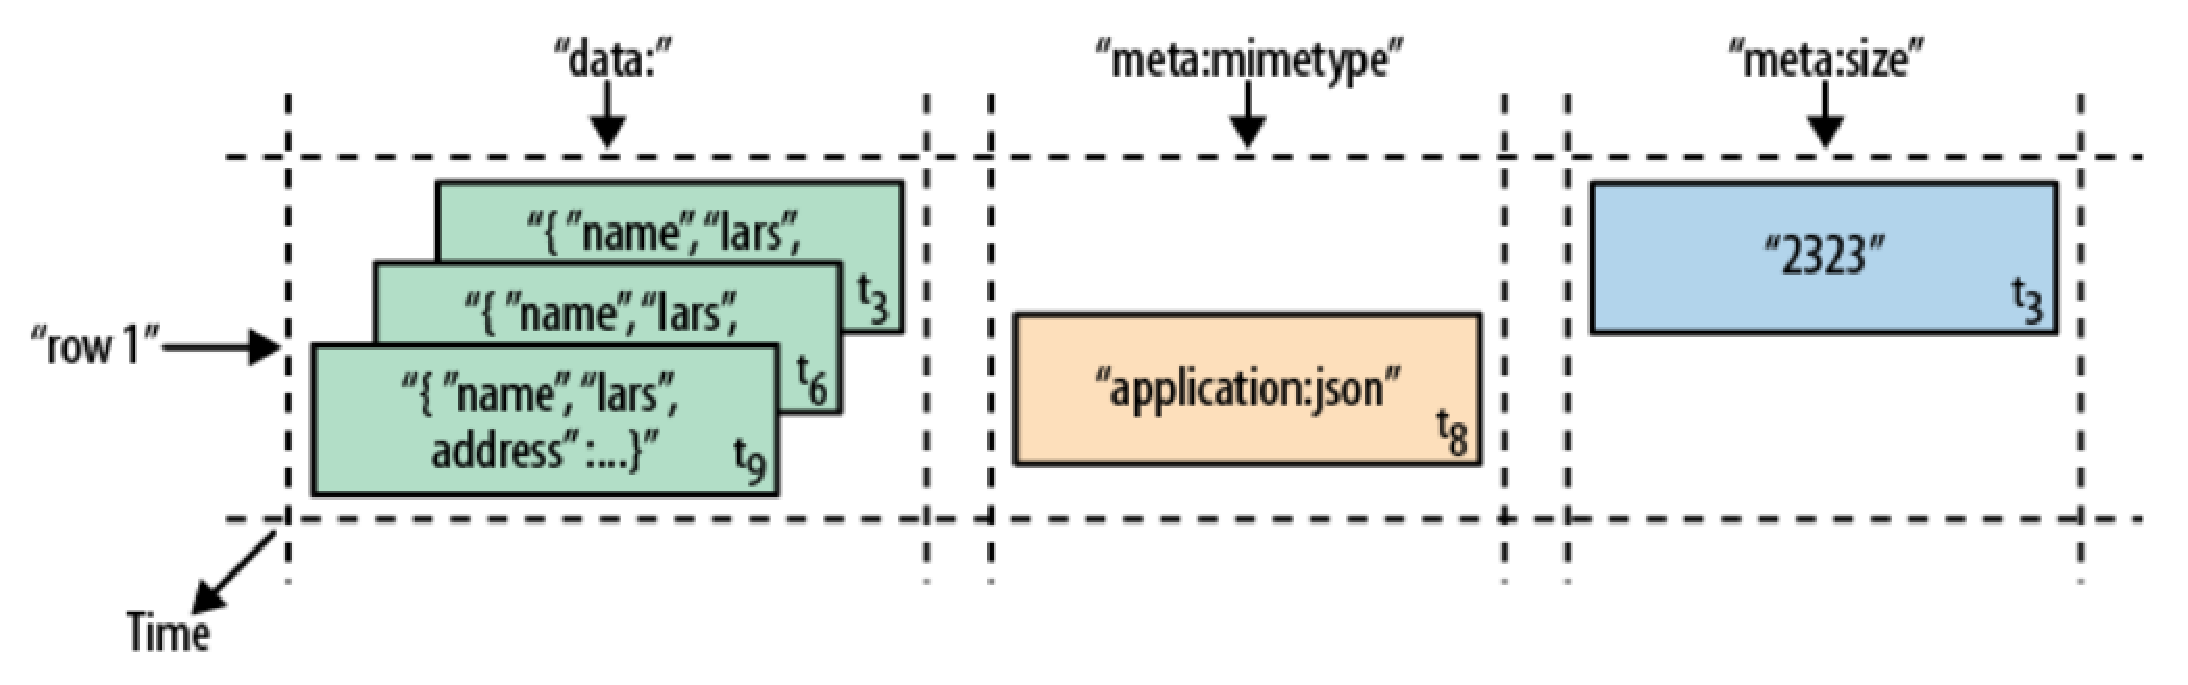
\includegraphics[keepaspectratio=true,scale=0.4]
	  {figuras/hbase-row.eps}
	\caption[Linha armazenada no HBase]{Linha armazenada no HBase
	\protect\linebreak Fonte: \cite{george2011}}
	\label{fig-hbase-row}
\end{figure}
\FloatBarrier

A figura \ref{fig-hbase-row} apresenta como uma linha está organizada em uma tabela composta por três colunas, duas delas agrupadas em uma família nomeada como \textit{meta}. Cada célula possui um identificador \textit{ti}, onde \textit{i} significa o tempo em que a célula foi escrita na tabela. A figura \ref{fig-hbase-table} ilustra este mesmo exemplo, porém representado em uma tabela.

\begin{figure}[ht!]
	\centering
	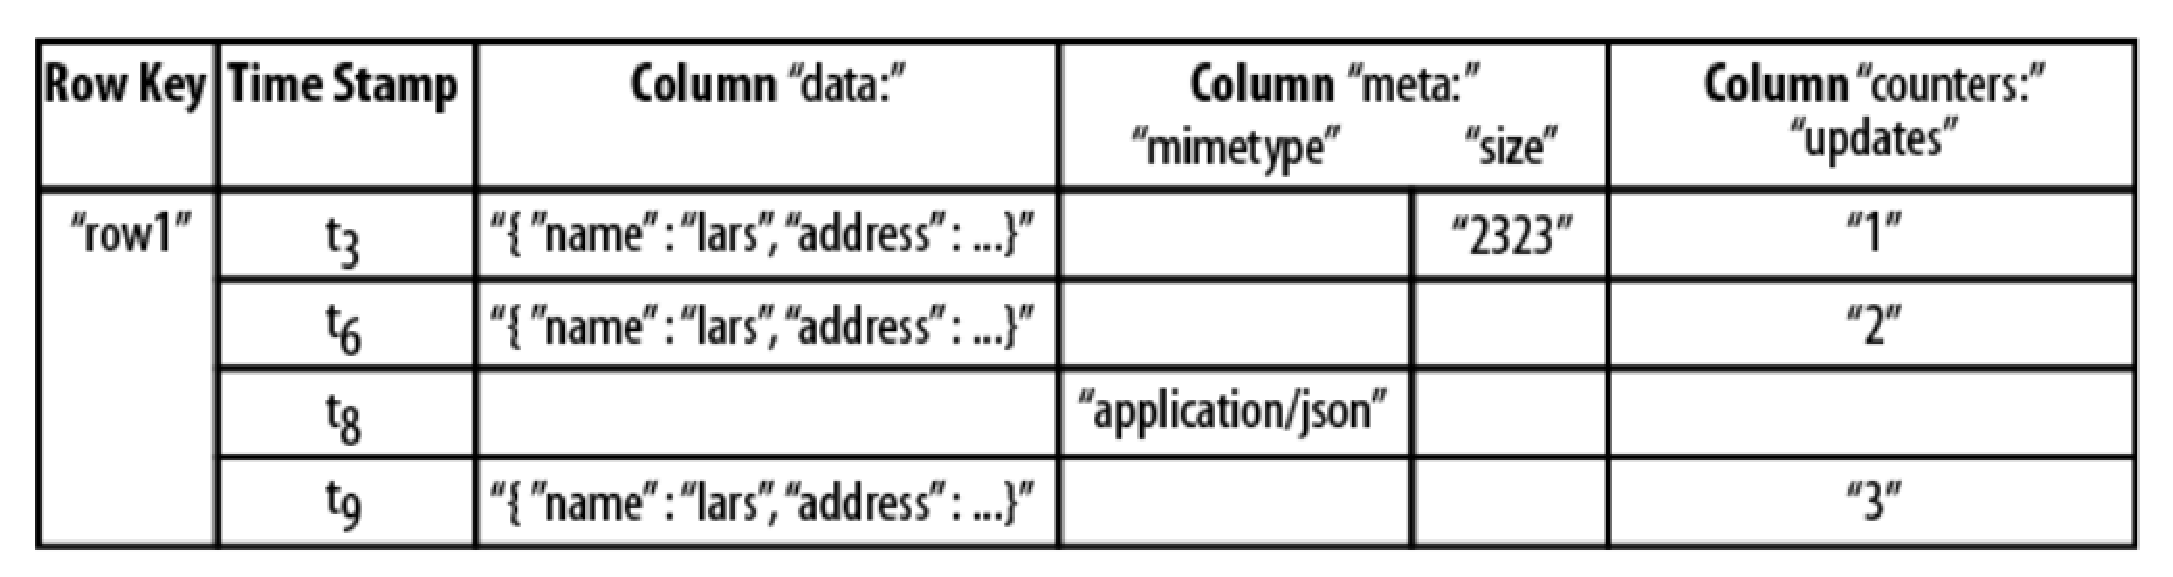
\includegraphics[keepaspectratio=true,scale=0.4]
	  {figuras/hbase-table.eps}
	\caption[Tabela HBase]{Tabela HBase
	\protect\linebreak Fonte: \cite{george2011}}
	\label{fig-hbase-table}
\end{figure}
\FloatBarrier

Uma das principais características do HBase pode ser identificada na sua capacidade para auto gerenciar sua base de dados. Segundo \citeonline{white2012} e \citeonline{george2011}, O conteúdo de todas as tabelas é automaticamente particionado e espalhado pelo \textit{cluster} em regiões distintas. Cada região é composta por um servidor que fica responsável por armazenar um intervalo de valores de uma determinada tabela. A figura \ref{fig-hbase-region} apresenta como uma tabela é dividida ao longo de regiões pelo HBase.

\begin{figure}[ht!]
	\centering
	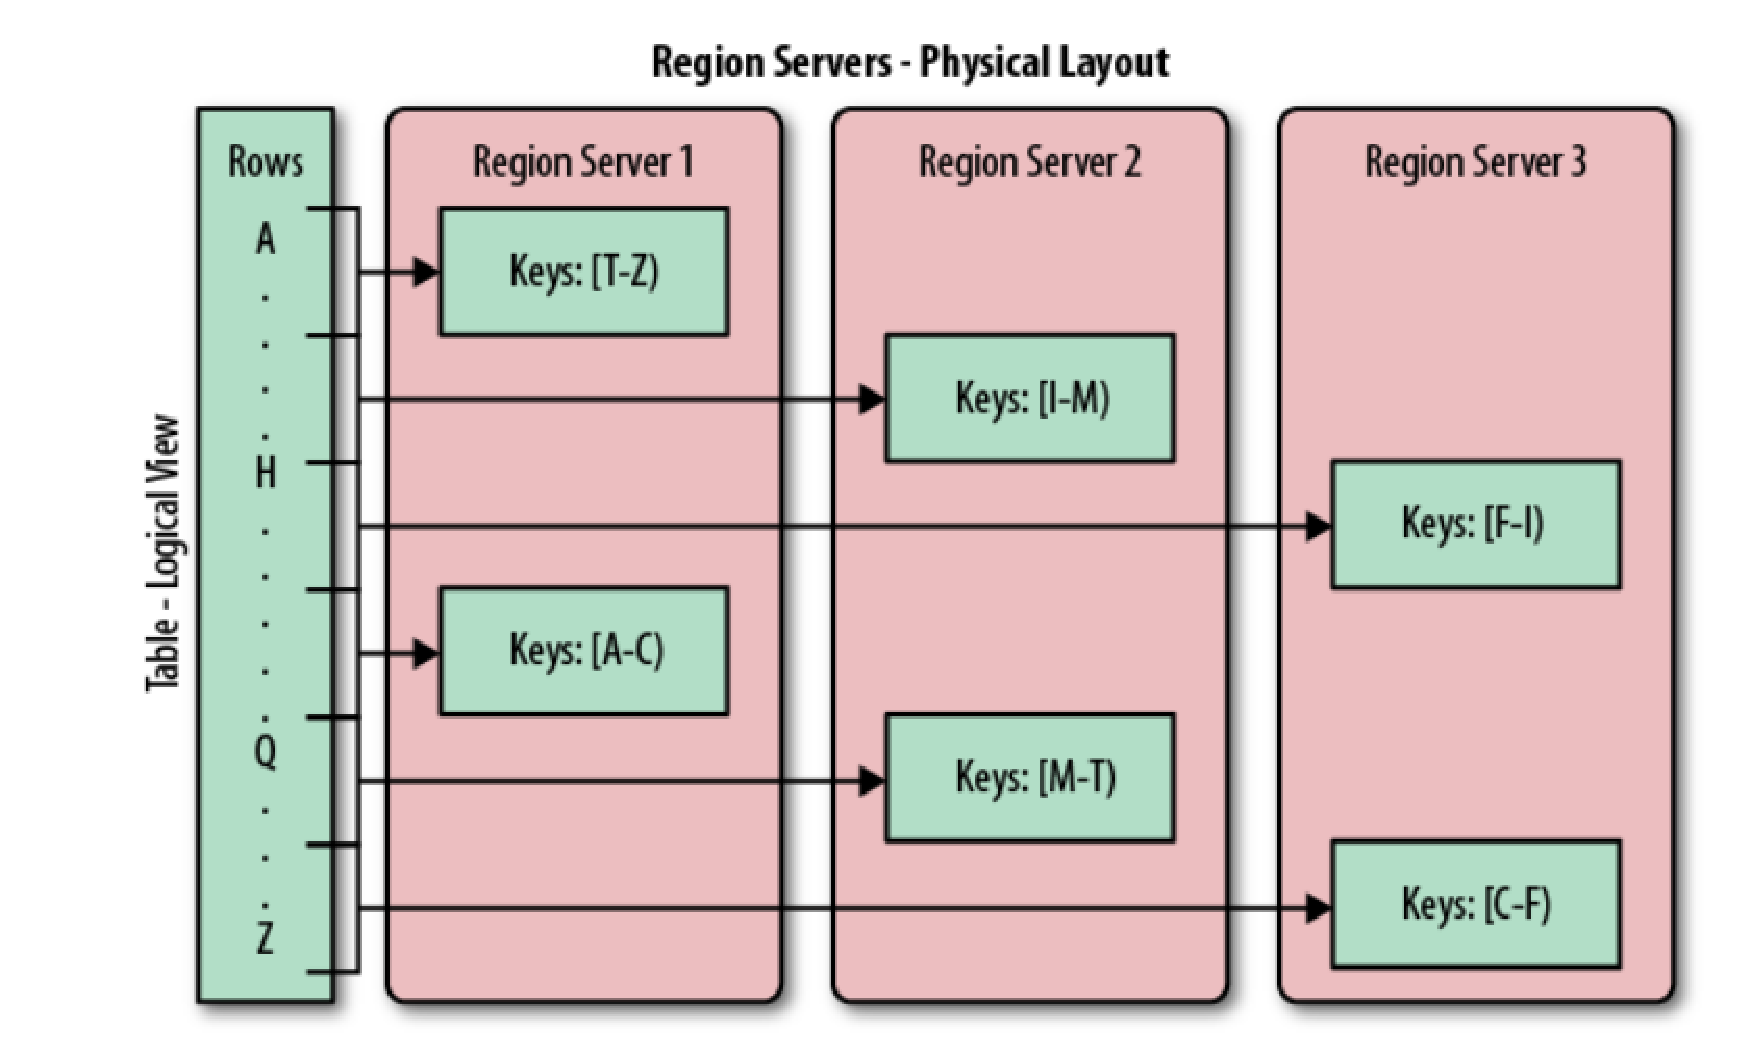
\includegraphics[keepaspectratio=true,scale=0.5]
	  {figuras/hbase-region.eps}
	\caption[Regiões HBase]{Regiões HBase
	\protect\linebreak Fonte: \cite{george2011}}
	\label{fig-hbase-region}
\end{figure}
\FloatBarrier

